\documentclass{article}
\usepackage{graphicx} % Required for inserting images
\usepackage{hyperref} % For url links
\usepackage{amsmath} % For math eqns
\usepackage{MnSymbol}
\usepackage{xcolor} % For coloring text (used for links)
\usepackage{csquotes}
\usepackage[style=ieee, backend=biber]{biblatex} 
\DeclareFieldFormat{sentencecase}{#1}
\addbibresource{our_bib.bib}


\title{Reinforcement Learning\\ \large{Midterm Report}}
\author{Mathias Øgaard \& Tobias Verheijen}
\date{April 2024}

\begin{document}

\maketitle

\tableofcontents

\section{Introduction}
The main focus of our project is to repeat the experiments performed in Application of reinforcement learning to the game of Othello \cite{vanEck2008}, aiming to implement an Othello-playing agent. This set of experiments will also be aided by the work of \cite{vdRee2013}\\
The environment which we will stage our agent against is given by a Python script \cite{codes} which has eight different Artificial Intelligence (AI) playing options for the Othello board game. In the van Eck and van Wezel experiment, they built two Q-learning agents who played against each other. For simplicity, we will have just one Q-learning agent play against the AI agents presented in \cite{codes} instead. For further information on the AI agents, please see section \ref{doc:env}.\\
The state space of Othello is far too large to run an exhaustive search for each state. Therefore, we will start by implementing one non-learning agent for benchmarking: \textit{The Positional Player} (section 4.1 in \cite{vanEck2008}). Please refer to section \ref{doc:env_agnts} of our analysis for a more elaborate description of the positional player. We will then implement a Q-learning agent (section 4.3 in \cite{vanEck2008}) and train it by staging it against the mentioned AI \cite{codes}.\\
As in \cite{vanEck2008}, after approximately $1,000,000$ games, we will let it play $100$ games against the non-learning player to measure its performance. This process is repeated until we reach the satisfying result of our agent being able to play Othello at a medium/high level. In an ideal world, it will improve against each of the 8 AI agents and will comprehensively beat the positional player used as a baseline.\\\\
Our report is outlined as follows: We first provide a description of the Othello board game and the environment, then we outline the algorithms which we will use for our analysis. We follow this with a summary of our preliminary experimental results, and we will close with a list detailing the plans for the remainder of our project.

\section{\label{doc:env}Environment}
\subsection{Othello Description}
A brief description of the Othello board game follows. Opponents with opposing colored discs alternate moves in an attempt to secure as many positions on an 8x8 board of their respective colors as possible. The winner is the player who has the most pieces when an end state is reached: When neither player can make a valid move or the board has no open spaces. A valid move is a move that flips a number of the opponent’s pieces by trapping them between your own pieces, like in the example in figure \ref{fig:valid_move}. 
\begin{figure}[ht] % ht places the image ish here in the text 
\centering
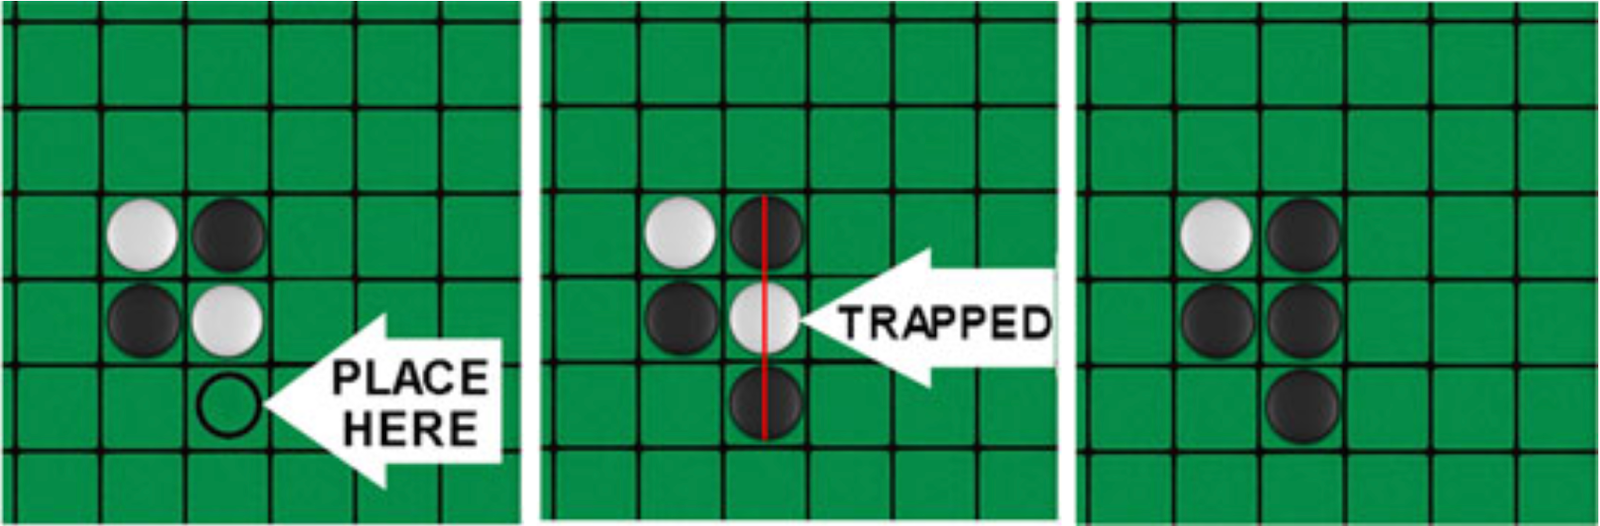
\includegraphics[width=0.75\linewidth]{valid_move.png}
\caption{\label{fig:valid_move}Example of a valid move. Taken from: \cite{picture}}
\end{figure}
\\The example shows only one tile trapped between the dark discs, however this can be extended so that several tiles are trapped between one players pieces. In this instance, all of the trapped tiles are flipped before the next player is able to make their move.

\subsection{\label{doc:env_desc}Environment Description}

The design of our environment takes into account a number of common pieces: the state space, the set of actions, and the transition function. There are also a number of situationally dependent portions: the reward, the utility, the policy, and the value function. The state is easily represented as the current state of the board, which considers the number of opposing discs, the number of our own discs, and the positions of each disc. The set of actions is simply the list of legal moves at a current state. The transition function is a deterministic function which indicates which discs will be flipped once an action has been played. The reward function for the positional agent is taken directly from the van Eck and van Wezel paper, and is given as a weighted sum of the value assigned to a position on the board and +1, 0, or -1 for whether the position is occupied by our own disc, empty, or our opponent’s disc respectively. In the end game, when either 80\% of the board is filled or all corner tiles are occupied, the reward function switches to maximizing the number of our discs and minimizing the number of our opponent’s discs. Since these are the only options considered by their models, the utility and policy functions are irrelevant to the decision making process \cite{vanEck2008}.

\subsection{\label{doc:env_agnts}Environment Agents}
We are using an environment for the Othello game \cite{codes}, containing one positional and eight different AI algorithms playing Othello:
\begin{itemize} 
    \item EvalBoard \textit{(positional player)}:   Returns the action giving the best next state, according to the EvalBoard() function (see section \ref{doc:env_func})
    \item Minimax:   Minimising the maximum loss, a.k.a. maximising the minimum reward.
    \item Minimax w/ Alpha-Beta Pruning:    Aims to decrease the number of potential moves evaluated
    \item Negamax:  Version of Minimax, utilising the fact that:
    \begin{equation*}
        Value(board, player 1) = -Value(board, player 2)
    \end{equation*}
    \item Negamax w/ Alpha-Beta Pruning
    \item Negascout (Principal Variation Search):  Extension of Negamax which aims to be faster than Negamax with Alpha-Beta Pruning by never considering nodes which wouldn’t be considered by Alpha-Beta Pruning and further reducing the search space.
    \item Minimax w/ Alpha-Beta Pruning w/ Sorted Nodes:    Prioritising high-valued moves when searching by making use of the GetSortedNodes() function (see section \ref{doc:env_func}).
    \item Negamax w/ Alpha-Beta Pruning w/ Sorted Nodes
    \item Negascout (Principal Variation Search) w/ Sorted Nodes 
\end{itemize}

\subsection{\label{doc:env_func}Environment Functions}
The environment provides us with a few native functions that we will take advantage of when implementing our playing agent\cite{codes}.
\begin{itemize}
    \item InitBoard(): Initialises the board in Othello starting position.
    \item PrintBoard(): Prints the current state of the board.
    \item MakeMove(): Assuming a valid move is provided, the agent makes the move at the specified position. Returns the board in its updated state and the count of how many tiles were flipped in the move-makers favour.
    \item ValidMove(): Checks if the move provided is valid. Returns boolean result
    \item EvalBoard(): Naively calculates the value of the board assuming corners are worth 4 points, edges are worth 2 points, and interior points are worth one point. The function returns the total board score.
    \item IsTerminalNode(): If there are no valid moves, the function returns true and marks the end of the game.
    \item GetSortedNodes(): Plays all possible moves for the agent and calculates the value of the board for each such move. Then the results are sorted in decreasing order: Highest valued moves first.
    \item BestMove(): Returns the best move according to the indicated playing agent.
\end{itemize}

\section{Description of the algorithms}
For our experiments, we will implement the Q-learning algorithm, as specified in section 2.1 of \cite{vanEck2008}:

\begin{figure}[ht]
\centering
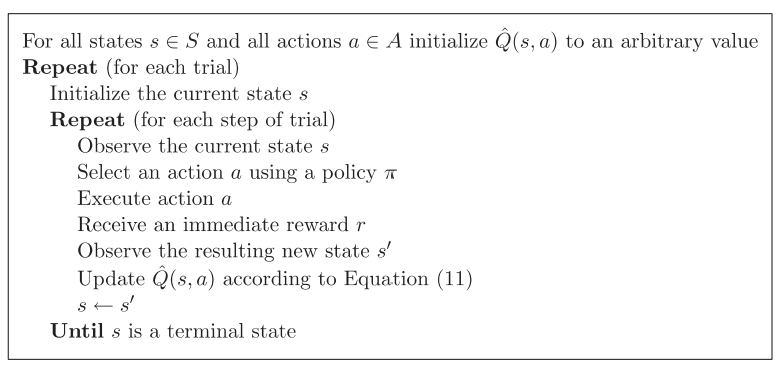
\includegraphics[width=0.85\linewidth]{Q_algo.png}
\caption{\label{fig:Q_algo}Pseudo-code for Q-Learning algorithm}
\end{figure}

\noindent Where Equation (11) is:

\begin{equation}
    \hat{Q}(s, a) \leftarrow (1-\alpha)\hat{Q}(s,a) + \alpha\left(r+\gamma \text{max}_{a'\in A}\hat{Q}(s', a')\right)
\end{equation}


\noindent The Q-Learning model will be a neural network similar to those outlined in class on April 16th. The input to the model will be a 64x1 column vector with 1s for positions where valid moves can be made after flattening the board and 0s where the model will not be able to play.
The neural network will output Q. 
The action is then chosen based on a weighted probability which considers the benefit of exploiting our current knowledge or exploring a new action to gain more knowledge of different moves. We can decrease the exploration rate over time, so that as we gain more information, we are more likely to exploit what we know rather than to explore different actions.

\section{Summary of preliminary experimental results}
In addition to the positional player described in section \ref{doc:env_agnts}, we have implemented a positional player which makes use of the position value matrix from \cite{vanEck2008} provided below in figure \ref{fig:pos_vals}.

\begin{figure}[ht]
\centering
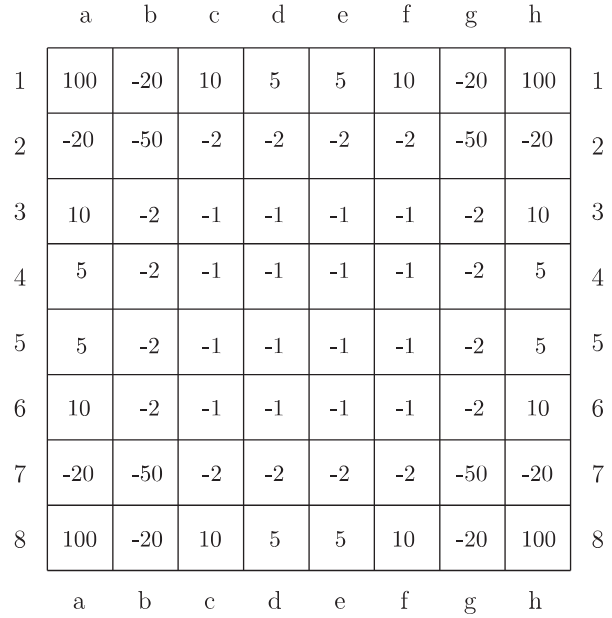
\includegraphics[width=0.6\linewidth]{position_vals.png}
\caption{\label{fig:pos_vals}Position Value Matrix as outlined in \cite{vanEck2008}.}
\end{figure}

In implementing the Q-Learning algorithm we have reached a point wherein we would like some feedback from you, the reader (\textit{hello})... \textbf{In the traditional Q-Learning algorithm, the model makes two moves, one in the original given state, and then another in the next state after taking its best action from the old Q function. However, in Othello it doesn't work to evaluate our agent making two consecutive moves. That is to say, the opponent would make a move between the two moves evaluated in the Q-Learning algorithm. How can we best incorporate this? Do we evaluate the opponents using our Q function and return a negative result? \textit{Some feedback on this portion would be extremely beneficial.}}\\
As somewhat inexperienced Othello players, we have found that it is relatively comforable to beat the \textit{Minimax} and \textit{EvalBoard} agents when playing individually against the agents. This indicates that they are good baselines for our Q-Learning algorithm as we will be able to see quickly if the model is improving or not.

\section{Plan for the remainder of the project}
\begin{verbatim}
    #TODO (optional): Do the project?
\end{verbatim}
\begin{enumerate}
    \item We will start by improving the interface to interact with the agents. This is important for human interpretation of the scenario.
    \item We will add an option to play on a reduced board size, e.g. 4x4, to allow for faster prototyping and evaluation of our algorithmic implementation.
    \item Implement our own Q-Learning player using code and algorithms from class.
    \item Run experiments on our Q-learning player to evaluate its performance
    \item Visualize our results
    \item Iteratively compare Q-Learning agent against base-line Positional Player implemented and described in section 3.
\end{enumerate}


% \section{References}
% \begin{itemize}
%     \item[1.] 	N. J. van Eck and M. van Wezel, ``Application of reinforcement learning to the game of Othello,'' Computers \& Operations Research, vol. 35, no. 6, pp. 1999–2017, Jun. 2008, doi: https://doi.org/10.1016/j.cor.2006.10.004. [Online]. Available \textcolor{blue}{\underline{\href{https://citeseerx.ist.psu.edu/document?repid=rep1&type=pdf&doi=ceec5e39fdd0c8be0e6270c46488ccfe0254a6b6}{here.}}}
%     \item[2.]	M. Van Der Ree and M. Wiering, ``Reinforcement Learning in the Game of Othello: Learning Against a Fixed Opponent and Learning from Self-Play.'' Accessed: Mar. 18, 2024. [Online]. Available \textcolor{blue}{\underline{\href{https://www.ai.rug.nl/~mwiering/GROUP/ARTICLES/paper-othello.pdf}{here.}}}
%     \item[3.]	``Reversi Othello $\llangle$ Python recipes $\llangle$ ActiveState Code,'' code.activestate.com. Accessed: Mar. 18, 2024. [Online]. Available \textcolor{blue}{\underline{\href{https://code.activestate.com/recipes/580698-reversi-othello/}{here.}}}
%     \item[4.]   ``Othello Reversi Online: Play Reversi Online Free,'' playpager.com, Accessed: Apr. 18, 2024. [Online]. Available \textcolor{blue}{\underline{\href{https://playpager.com/othello-reversi/}{here.}}}
% \end{itemize}

% This is a sample text to showcase the citations and bibliography in the style of IEEE with biblatex. After this sentence, three journal articles are cited 
% The following citations refer to a book \cite{codes}, \cite{vanEck2008}, \cite{vdRee2013}, \cite{picture}
% a book chapter \cite{Keller2022} and to a PhD thesis \cite{Hautle2023}. Finally, this is an example of a conference proceeding \cite{Iqbal2023} and this is a citation of several references at once \cite{Iqbal2023,Hautle2023, Keller2022, Aad2015}
\newpage
\printbibliography

\end{document}
